\documentclass[Master,MSE,german]{twbook}
\usepackage[utf8]{inputenc}
\usepackage[T1]{fontenc}
\newcommand{\FHTWCitationType}{IEEE}
\usepackage{bibgerm}
\usepackage{float}
\usepackage{eurosym}

% Definition Code-Listings Formatierung:
\usepackage[final]{listings}
\lstset{captionpos=b, numberbychapter=false,caption=\lstname,frame=single, numbers=left, stepnumber=1, numbersep=2pt, xleftmargin=15pt, framexleftmargin=15pt, numberstyle=\tiny, tabsize=3, columns=fixed, basicstyle={\fontfamily{pcr}\selectfont\footnotesize}, keywordstyle=\bfseries, commentstyle={\color[gray]{0.33}\itshape}, stringstyle=\color[gray]{0.25}, breaklines, breakatwhitespace, breakautoindent}
\lstloadlanguages{[ANSI]C, C++, [gnu]make, gnuplot, Matlab}

\makeatletter
\renewcommand\lstlistingname{Quellcode}
\renewcommand\lstlistlistingname{Quellcodeverzeichnis}

% Definition des Macros listoflolentryname analog zu listoflofentryname und listoflotentryname der KOMA-Klasse
\newcommand\listoflolentryname\lstlistingname
% Neudefinition der Zeilen des Quellcodeverzeichnisses wenn die Option listof=entryprefix gewählt wurde
\@ifclasswith{scrbook}{listof=entryprefix}
{%
    \renewcommand\l@lstlisting[2]{\@dottedtocline{1}{1.5em}{1em}{\listoflolentryname~#1}{#2}}
}{%
}
\makeatother
\newcommand{\listofcode}{\phantomsection\lstlistoflistings}

%
% Einträge für Deckblatt, Kurzfassung, etc.
%
\title{Architekturerstellung auf Basis von Anforderungen}
\author{Bernhard Posselt, BSc}
\studentnumber{1310299032}
\supervisor{Mag. Maria-Therese Teichmann}
\place{Wien}
\kurzfassung{sehr kurz}
\schlagworte{Schlagwort1, Schlagwort2, Schlagwort3, Schlagwort4}
\outline{abstract da}
\keywords{Keyword1, Keyword2, Keyword3, Keyword4}

\begin{document}


\maketitle

%
% .. und hier beginnt die eigentliche Arbeit. Viel Erfolg beim Verfassen!
%

\chapter{Einführung}

\section{Motivation}
\subsection{Wie kommt man von Anforderungen auf eine gute Architektur}
Vermutung: Gute Architektur häng von guten Anforderungen ab, deswegen muss Anforderungsprozess erweitert werden
Probleme aufzählen die bei einer schlechten Architektur entstehen.

vielleicht noch genauer spezifizieren dass es keine all round solution werden soll sondern die meisten use cases abdecken soll (grafik wieviel apps SOA haben zb)

\subsection{Gibt es eine Art Kochrezept für die Architekturerstellung}
Gesucht: Ein Prozess mit dem auf die wichtigen Faktoren eingegangen werden kann.

\section{Was wird gemacht}
\subsection{Planung einer Zertifizierungsstellen Architektur}
\subsection{Modellierung mit UML}
\subsection{Anpassen der Anforderungestemplates}
\subsection{Architekturplanung Prozesserstellung, eine Art Framework}
\subsection{Dokumentation der Prozesserstellungsanläufe}

\section{Was wird nicht gemacht}
\subsection{Abdeckung des kompletten Prozesses}
Weil zu umfangreich, genauere Beschreibung im Architektur kapitel, auch erklären dass es sich heraus gestellt hat dass man nicht alles sofort planen und bewerten kann wegen fehlenden Messmöglichkeiten
\subsection{Kein Organisations- und Kommunikationsmanagement}
\subsection{Implementation}
Zu umfangreich
\subsection{Abdeckung aller möglichen Architekturfälle (Embedded, High Performance)}
\subsection{Abdeckung aller möglichen Archtekturreviewmethoden}
\subsection{Komplette Vorgaben der Bewertungs-Methoden}
Eher Hinweise auf wie man zb Ausfallkosten bewerten könnte, Methode auf eigene Anwendungsfälle abänder- und ersetzbar. Aber aufzeigen warum es gut sein kann sie dennoch schon zu behandeln
\subsection{Kompletter Anforderungsprozess}
Nur eine Erweiterung im Hinblick auf benötigte Parameter

\section{Übersicht}
Erklären was in welchen Kapiteln behandelt wird
\subsection{Modellierung}
\subsection{Anforderungen}
\subsection{Architektur}
\subsection{Prozesserstellung}
\subsection{Prozessumsetzung Anforderungen}
\subsection{Prozessumsetzung Architektur}
\subsection{Zusammenfassung}


\chapter{Modellierung}
Kurze Einführung in die Modellierung. Warum ist sie wichtig, was wird verwendet. Die wichtigsten Grundsachen erklären und erklären für was welcher Diagrammtyp verwendet wird

\section{Warum ist Modellierung wichtig}
\section{Was ist UML}

\section{Diagrammtypen}
\subsection{Kontextdiagramm}
\subsection{Komponentendiagram}
\subsection{Klassendiagramm}
\subsection{Aktivitätsdiagramm}
\subsection{Usecasediagramm}


\chapter{Anforderungen}
Behandeln der ISO 9126 Anforderungen, versuchen zu erklären was man alles beachten muss und was überhaupt ab anfang messbar ist (z.B. performance nicht messbar)

\section{Funktionale Anforderungen}
Wichtig: Security ist eine funktionale Anforderung

\section{Nicht funktionale Anforderungen}
\subsection{Reliability}
\subsection{Usability}
\subsection{Efficiency}
\subsection{Maintainability}
\subsection{Portability}

\chapter{Architektur}
Erklären generell was Software Architektur ist und mit was sie sich beschäftigt

\section{Architekturprozess Lifecycle}
Diagramm wie der Architekturprozess im groben abläuft. Dann den Teil markieren auf dem der Fokus der Arbeit liegt

\section{Was ist eine gute Architektur}
Zitate; Architektur ist ein abwägen von Vor- und Nachteilen. Es gibt keine perfekte Architektur, jede Entscheidung ist mit Vor und Nachteilen versehen.

\section{Architekturbewertungsmethoden}
Kurze Einführung in Architekturbewertungsmethoden

\subsection{ATAM}
\subsection{CBAM}

\chapter{Prozesserstellungsversuche}
Der Architekturprozess ist komplex und ein falsches Vorgehen kann der Ursprung vieler Probleme sein \cite[S. 7-8]{softarch}. Deswegen ist es notwendig einen eigenen Prozess zu definieren, welcher die Erstellung vereinfacht und die Fehlerkosten minimiert. Dieser Prozess sollte schon in der Planungsphase zum Einsatz kommen, da hier wegen der Zehner-Regel der Fehlerkosten der größte Effekt zur Reduzierung der Fehlerkosten erzielt werden kann \cite[S. 154]{fehler}.

Der Prozess wurde anhand eines Beispielprojektes erstellt und dreht sich um die Architektur eines Systems einer Personenzertifizierungsstelle.

\section{Vorhandene Daten}
Ausgegangen wurde von folgenden Anforderungsdokumenten, welche in der Erstellung des Prozesses mehrfach abgeändert und an die Architekturprozessanforderungen angepasst wurden:

\begin{itemize}
  \item Usecasediagramm: modelliert die Usecases des Unternehmens
  \item Usecasebeschreibung: ausgefülltes Anforderungstemplate, welches Sonderfälle, nicht funktionale Parameter und weitere Details beinhaltet
  \item Klassendiagramm: visualisiert die zu verwendeten Daten
  \item Aktivitätsdiagramme: visualisiert den Ablauf komplexerer Usecases
  \item Kontextdiagramm: zeigt die Datenflüsse zwischen AkteurInnen, Nachbarsystemen und dem zu erstellenden System
  \item ISO Anforderungsdokument für Personenzertifizierungsstellen \cite{ISO_CERT}: beschreibt die Rahmenbedingungen für den Betrieb einer Personenzertifizierungsstelle
\end{itemize}

\section{Prozesserstellungsversuche}
Ausgehend von den vorhandenen Daten wurden mehrere Prozesse definiert, welche bis auf den Letzten entweder zu grobe Ergebnisse lieferten, oder nicht nachvollziehbar waren.

Ausgangsbasis war eine Systemvision mit folgenden Anforderungen:

\begin{itemize}
  \item Es soll eine Webseite entstehen, welche die Prüfungstermine auflistet und Personen erlaubt, sich für diese Prüfungen anzumelden. Dadurch soll der Verwaltungsaufwand reduziert werden, um Kosten zu sparen.
  \item Die Übermittlung der Prüfungsdaten soll über einen eigenen VPN Server geschehen, um die Datensicherheit des Systems zu erhöhen.
  \item Die Prüfungsdaten werden firmenintern verwaltet und nach der Auswertung soll der Scheme Owner benachrichtigt werden. Beide Usecases sollen auf eine sichere Art und Weise umgesetzt werden.
\end{itemize}

\begin{figure}[!htbp]
    \centering
    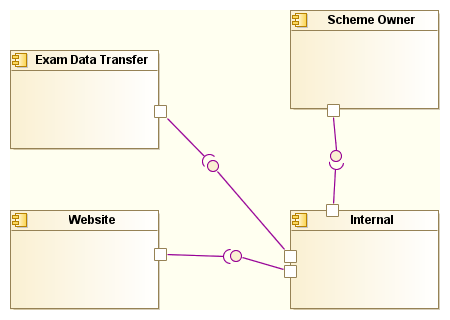
\includegraphics[scale=0.6]{uml/vision.png}
    \caption{Systemvision der Komponenten}
\end{figure}

Aufbauend darauf wurde dann versucht einen Prozess zu finden, der diese Grundideen berücksichtigt.

Die anfänglichen Versuche basierten stark auf einem ATAM Utility Tree ähnlichen Verfahren, bei welchem die nicht funktionalen Anforderungen nach der Formel von Oliver Vogel priorisiert wurden: \glqq Priorität = (Nutzen + Risiko + Wirkung) / 3\grqq \cite[S. 374]{softarch}. Die Bewertung der Komponenten wurde auf Basis einer bestehenden Tabelle mit Basisarchitekturen abgeleitet \cite[S. 179]{review}.


\subsection{Vom Usecase zur Komponente durch Priorisierung der nicht funktionalen Anforderungen}
Der erste Versuch zur Erstellung des Architekturprozesses orientierte sich am Prinzip: teile und herrsche. Der Prozess verwendete aufgrund der initialen Vermutung, dass nicht funktionalen Anforderungen die Hauptentscheidungsbasis für die Architektur darstellen, eine priorisierte Liste von nicht funktionalen Anforderungen. Danach wurde versuchte, anhand der priorisierten Anforderungen passende Komponenten auszuwählen. Der Ablauf war folgender:

\begin{itemize}
  \item Für jeden Usecase wird ein komplettes Komponentendiagramm des Systems erstellt.
  \item Die Komponenten jedes Teilsystems werden anhand ihrer nicht funktionalen Qualitäten aus einem Pool von Komponentenarchitekturen gewählt. Diese Komponentenarchitekturen beinhalteten zB. Systeme wie den üblichen Webstack, welcher sich aus Komponenten wie dem Loadbalancer, Datenbankserver, Applikationsserver und Webserver zusammensetzt.
  \item Schlussendlich werden alle Teilsysteme miteinander vereinigt, soweit es die nicht funktionalen Attribute erlauben.
\end{itemize}

Dieser Prozess scheiterte nicht nur am enormen Modellierungsaufwand, sondern auch am Auswahlprozess der Komponentenarchitekturen: Je nachdem, welche Komponentenarchitekturen vorhanden waren und wie diese bewertet wurden, entstanden unterschiedliche Architekturen. Zudem schien es zu viele Komponentenarchitekturen zu geben, da einzelnen Komponenten beliebig miteinander kombinierbar waren.

Die Qualität der Architektur hätte folglich von der Vollständigkeit dieser scheinbar unendlich großen Menge an Komponentenarchitekturen abgehangen. Aus diesem Grund schien der Prozess ungeeignet für die Architekturerstellung und wurde somit verworfen.

\subsection{Von einer Architektur mit hoher Kohäsion und anschließendem Architekturreview zu den Komponenten}
Um das Problem des sehr hohen Modellierungsaufwandes des ersten Prozesses zu umgehen, wurde von einer Grundarchitektur mit hoher Kohäsion ausgegangen. Diese Komponentenarchitektur entstand zusammen mit dem/der AuftraggeberIn, um zusätzliche Risiken indentifizieren zu können.

\begin{figure}[!htbp]
    \centering
    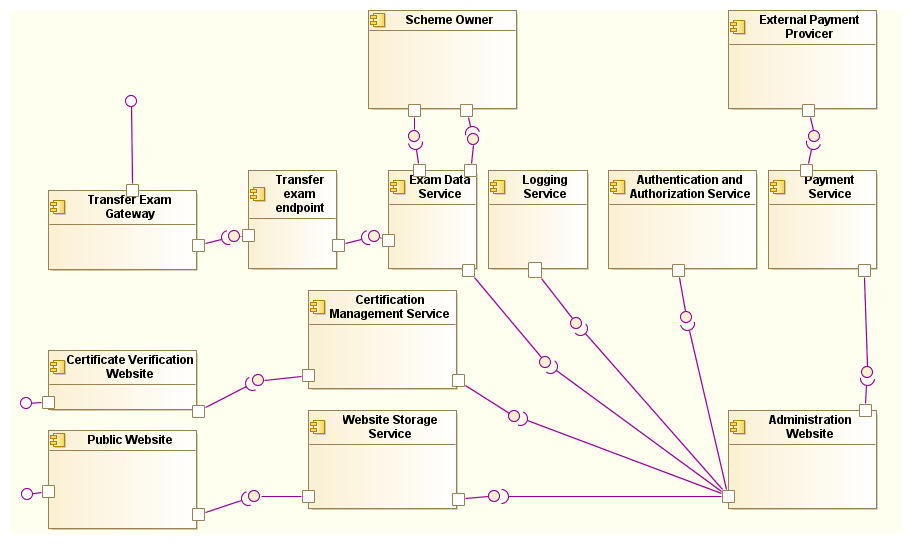
\includegraphics[scale=0.5]{uml/vision2.png}
    \caption{Architektur mit hoher Kohäsion}
\end{figure}

Diese Architektur sollte nun auf die Erfüllung der nicht funktionalen Anforderungen überprüft und gegebenenfalls angepasst werden. Zur Überprüfung der Anforderungen wurden die priorisierten, nicht funktionalen Anforderungen eines Usecases herangezogen. Der Prozess ähnelte damit stark einem szenariobasierten Review wie er in ATAM durchgeführt wird.

Auch dieser Prozess litt jedoch unter dem Problem, dass die nicht funktionalen Anforderungen schwer bewertet werden konnten. Außerdem war es schwer ein Regelwerk/Rezept aus der Architekturerstellung abzuleiten, da durch die Einbeziehung unterschiedlicher AuftraggeberInnen jeweils verschiedene Architekturen entstehen können. Die Einbeziehung von Kohäsion als Aufteilungsgrundlage der Komponenten verursachte zudem ein gefühlt zu großes System, welches in der Umsetzung sehr teuer geworden wäre. Die Kostenersparnis des Systems, welche in der Systemvision definiert wurde, schien damit unzureichend erfüllt zu werden.

\subsection{Von den Daten zu den Komponenten}
Die Auswahl und Bewertung der Komponentenarchitekturen und der starke Fokus auf die nicht funktionalen Anforderungen in den beiden vorherigen Prozessen stellte ein wesentliches Hindernis zur Erstellung eines eindeutigen Regelwerkes dar: Eine vollständige Auflistung aller möglichen Komponentenarchitekturen erschien entweder unmöglich oder unvollständig zu sein; eine Bewertung der nicht funktionalen Attribute schien ohne entsprechende Implementation nur sehr grob überprüfbar zu sein. Der Versuch, ein System mit hoher Kohäsion zu erstellen, endete zudem in sehr teuren Architekturen.

Dies war überraschend, da die populärste Architekturbewertungsmethode, ATAM, stark auf nicht funktionale Anforderungen aufbaute. Als Grund für diese Inkompatibilität wurde der Zeitpunkt der Architekturerstellung vermutet: Durch die fehlende Implementationsphase waren die nicht funktionalen Anforderungen sehr schwer zu bewerten und somit mehr oder weniger nicht überprüfbar. Deshalb wurden sie als Hauptkriterium und Ausgangspunkt für die Architekturerstellung verworfen.

Stattdessen wurde der Fokus auf die Aufspaltung der Daten gelegt. Die Daten wurden anhand Ihrer Vertraulichkeit in unterschiedliche Netze aufgeteilt. Diese Netze wurden dann durch Komponenten miteinander verbunden, die den Zugriff auf die Daten regelten.

\begin{figure}[!htbp]
    \centering
    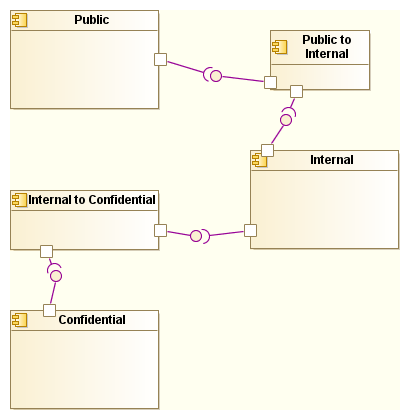
\includegraphics[scale=0.7]{uml/vision3.png}
    \caption{Aufteilung der Komponenten in Datenbereiche}
\end{figure}

Dieser Prozess erlaubte es, eine nachvollziehbare Architektur zu erstellen, jedoch war das Ergebnis zu grob. Außerdem schien eine separate Komponente zur  Übertragung der Prüfungsdaten zu fehlen, welche in der ursprünglichen Systemvision definiert und als notwendig empfunden worden war, um die Rahmenbedingungen der Vertrautheit zu erfüllen \cite[7.3]{ISO_CERT}.

\subsection{Von den Daten und den AkteurInnen zu den Komponenten}
Aufbauend auf dem vorherigen Prozess, welcher die Architektur anhand der Daten erstellte, wurden nun auch AkteurInnen eingebunden und deren Beziehungen zu den Daten ermittelt. Anhand dieser Beziehungen wurden Regeln erstellt, aus denen wiederum die Architektur erstellt wurde.

\begin{figure}[!htbp]
    \centering
    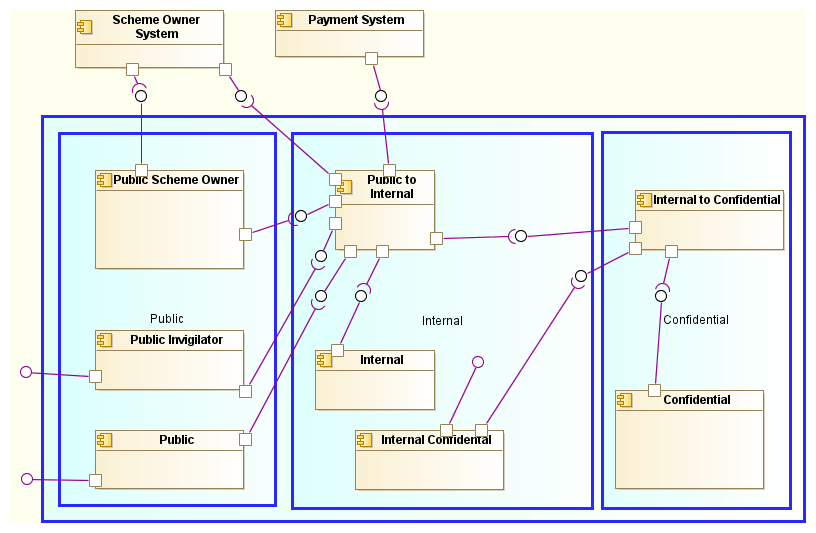
\includegraphics[scale=0.55]{uml/vision4.png}
    \caption{Aufteilung der Komponenten in Datenbereiche und AkteurInnen}
\end{figure}

Dieser Prozess schien nicht nur die Rahmenbedingungen und Sicherheitsbedingungen abzudecken, er war auch durch die erstellten Regeln nachvollziehbar und genau genug, um bereits einen guten Überblick auf die Architektur zu erlangen. Anhand der daraus resultierenden Architektur war es nun auch möglich, nicht funktionale Attribute wie zB. Antwortzeiten besser einschätzen zu können.

\chapter{Prozess Anforderungen}
Da die Software Architektur auf den Anforderungen basiert und viel wichtiger \glqq den gestalterischen Spielraum des Architekten\grqq \cite[S. 103]{softarch} begrenzt, kann davon abgeleitet werden, dass sowohl die Qualität der Architektur als auch die Akzeptanz des Systems wesentlich von den bereits im Vorfeld ermittelten Parametern abhängt. Das bedeutet wiederum, dass für die Klärung der Ausgangsfrage - Wie kommt man von Anforderungen auf eine gute Architektur - auch der Anforderungsprozess eine wichtige Rolle spielt.

Da der Anforderungsprozess ein an sich eigenes, sehr großes Themengebiet dar stellt, wird hier jedoch nur auf die Ausgangsartefakte eingegangen, welche später im Architekturprozess referenziert werden.

\section{Ermittlung der Usecases}
Die Usecases werden zusammen mit dem/der Kundin ermittelt. Daraus wird schlussendlich ein Usecase Diagramm erstellt, welches alle Akteure und Nebensysteme beinhaltet. Dies ist wichtig für das Kontextdiagramm, welches auch im Anforderungsprozess erstellt wird und die Ausgangsbasis für die Architektur dar stellt.

\begin{figure}[!htbp]
    \centering
    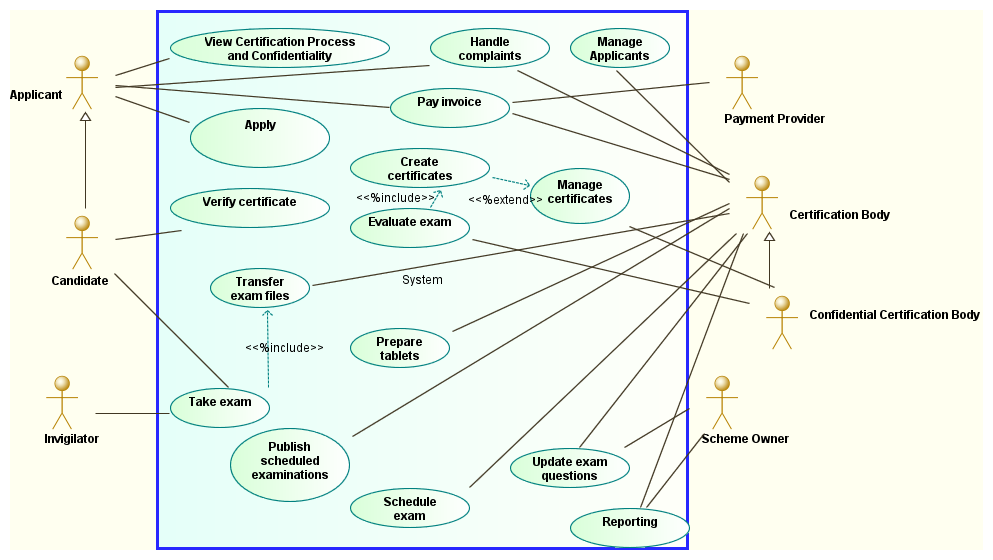
\includegraphics[scale=0.4]{uml/usecase.png}
    \caption{Das mit dem Kunden ermittelte Usecase Diagramm}
\end{figure}

\subsection{Erweiterte Dokumenation der Usecases}
Parallel zur Erstellung des Usecase Diagramms werden zusätzliche Parameter und Beschreibungen für jeden Usecase aufgenommen, welche im eigentlichen Diagramm keine Erwähnung finden.
Dafür wird ein Anforderungstemplate, auch Usecase Beschreibung genannt, verwendet \cite[S. 214]{reqman}, welches aufbauend auf einer Grundversion \cite[Abbildung 8.14, S. 215]{reqman} für jeden Usecase folgende Angaben aufnimmt:

\begin{itemize}
  \item Id: eine eindeutige Bezeichnung, welche dafür verwendet wird, um den Usecase zu referenzieren
  \item Actor: eine Auflistung aller Teilnehmer des Usecases
  \item Description: eine kurze Beschreibung des Usecases
  \item Preconditions: eine Auflistung von Vorbedinungen für den Usecase
  \item Postconditions: eine Auflistung von Nachbedingungen für den Usecase
  \item Normal Course of Events: eine Beschreibung des Standardablaufes
  \item Alternative Courses: Auflistung von Erweiterungen oder zusätzlichen Möglichkeiten
  \item Exceptions: Beschreibung von diversen Ausnahmefälle
  \item Assumptions: Annahmen, unter welcher der Usecase beschrieben wird
  \item Priority: eine Gewichtung, wie wichtig der Usecase ist
  \item Notes: sonstige Anmerkungen
\end{itemize}

Sind die Abläufe komplexer, können Aktivitäts Diagramme verwendet werden, um komplexere Abläufe verständlicher dar zu stellen \cite[S. 215]{reqman}:

\begin{figure}[H]
    \centering
    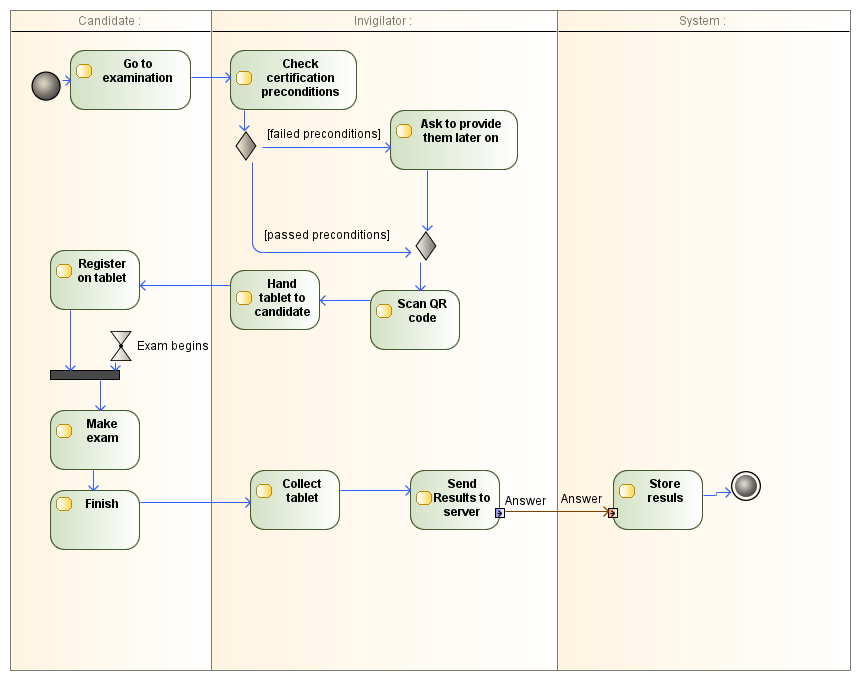
\includegraphics[scale=0.4]{uml/takeexamreq.png}
    \caption{Der Ablauf des Take Exam Usecases im Detail}
\end{figure}

\subsection{Einbeziehen von Architekturreviewparametern}
Um die Einhaltung der Qualitätsparameter zu garantieren, können Architekturreviews durchgeführt werden \cite[S. 20]{review}. Es existiert zwar \glqq keine singuläre, allgemein akzeptierte Metrik um eine Architektur zu beurteilen\grqq \cite[S. 19]{review}, jedoch liefern sie grobe Einschätzungen über die Angemessenheit des Systems \cite[S. 20]{review}. Folgende Architekturreviews wurden dafür ausgewählt:

\begin{itemize}
  \item ATAM: betrachtet Wachstums- und explorative Szenarien um die Architektur zu beurteilen \cite[S. 61]{review}
  \item CBAM: basiert auf ATAM, beachtet jedoch vor allem den Nutzen und die Risiken und Kosten der Architketur, um die Architekturentscheidungen besser abwähgen zu können. Hauptfaktor ist der ROI. \cite[S. 67]{review}
\end{itemize}

Für diese Reviews können bereits früh ein Großteil der benötigten Parameter ermittelt bzw. zumindest grob abgeschätzt werden. Dies ist wichtig, weil nach der 10er Regel der Fehlerkosten früh erkannte Fehler und Probleme weniger Kosten nach sich ziehen als später Erkannte \cite[S. 154]{fehler}.

Deswegen wird das Anforderungstemplate um folgende Parameter erweitert:

\begin{itemize}
  \item Earned Value per month: Wieviel Umsatz der Usecase in einer bestimmten Zeit generiert
  \item Expected Usage: Anzahl der erwarteten Nutzer des Systems pro Zeiteinheit
  \item Growth Scenarios: Anzahl der erwarteten Nutzer des Systems pro Zeiteinheit bei einer höheren Nutzeranzahl
  \item Change Scenarios: mögliche Änderungsszenarien und Erweiterungen
\end{itemize}

\subsection{Einbeziehen von nicht funktionalen Qualitätsattributen}
Nicht funktionale Qualitätsattribute beschreiben die nicht funktionalen Anforderungen an das System. Da Qualität oft schwammig formuliert ist, ist es wichtig, diese Attribute messbar zu machen \cite[S. 9]{effektiv}.

Deswegen werden für jeden Usecase und dessen architekturrelevanten, nicht funktionalen Anforderungen messbare Parameter definiert. Diese Parameter helfen schon im Vorfeld dabei die Architektur zu überprüfen.

Für das Beispielprojekt wurden folgende Parameter definiert, mit welchen das Anforderungstemplate erweitert wurde:

\begin{itemize}
  \item Response Time in Seconds: Wie schnell die Antwort des Systems auf eine Anfrage reagieren muss
\end{itemize}

\section{Rahmenbedingungen}
Zusätzlich zu funktionalen und nicht funktionalen Anforderungen werden auch die Rahmenbedingungen ermittelt, unter welchem das System erstellt werden soll. Diese Anforderungen beinhalten meist den organisatorischen und zeitlichen Ablauf des Projektes und können auch gewisse Technologien vorschreiben, zB. wenn das System in ein bereits bestehendes System integriert werden soll. \cite[S. 9]{review}\cite[S. 110]{softarch}

Die Rahmenbedingungen des Beispielprojektes lassen sich zum Großteil aus dem ISO Standard für Zertifizierungsstellen ermitteln \cite{ISO_CERT} und geben Einsicht in die Vertraulichkeit der Daten und eröffnen weitere Usecases. Sofern möglich werden diese Parameter in das Usecase Diagramm und das Klassen Diagramm der zu verwendeten Daten mit einbezogen. Auf zeitliche und technologische Rahmenbedingungen wurde im Beispielprojekt nicht eingegangen.

\section{Ermittlung der Daten}
Die zu speichernden Daten werden ermittelt und mit Hilfe eines Klassen Diagrammes modelliert. Dies ist nicht nur wichtig und nützlich, weil die Beispielanwendung in diesem Falle eine stark datenzentrierte Anwendung ist \cite[S. 105]{effektiv}, sondern wird später auch einen wesentlichen Beitrag zur Aufteilung des Systems in Komponenten leisten. Im Falle des Beispielprojekts wurden folgende Daten ermittelt und modelliert:

\begin{figure}[H]
    \centering
    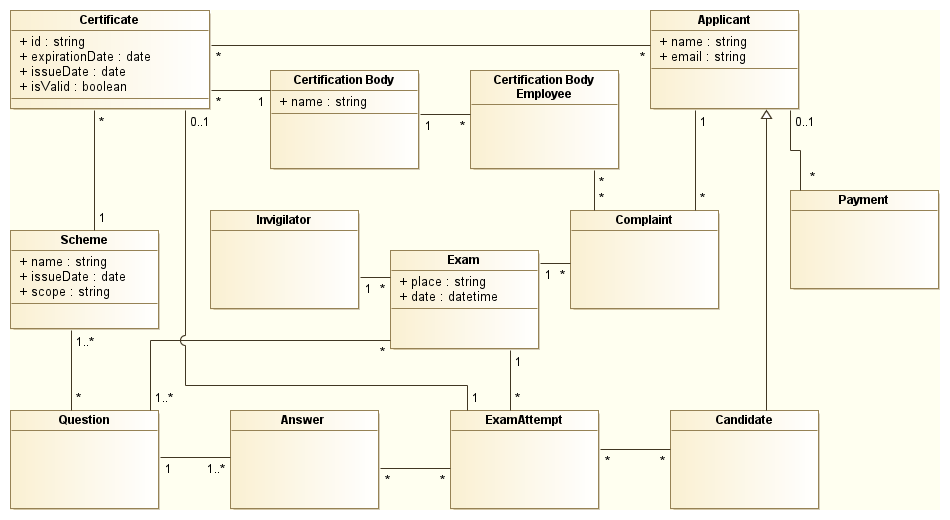
\includegraphics[scale=0.5]{uml/class.png}
    \caption{Das ermittelte Klassendiagramm des Beispielprojektes}
\end{figure}

\section{Ermittlung der Datenvertrautheit}
Nach der Ermittlung der Daten wird auf Basis der Rahmenbedingungen und Sicherheitsstruktur zusammen mit dem/der Kunden/Kundin ermittelt, welche Daten in welche Vertrautheitskategorien fallen. Dazu werden die Daten anhand ihrer gewollten Lesbarkeit in mehrere Untergruppen unterteilt.

Ermittelt wurden in diesem Falle folgende drei Kategorien:

\begin{itemize}
  \item Public: öffentlich zugängliche Daten, welche auf der Webseite zugänglich gemacht werden
  \item Internal: Daten, welche für die inneren Abläufe Betriebs notwendig sind, aber nicht öffentlich zugänglich sein sollen
  \item Confidential: Daten, welche innerhalb des Betriebes verwendet werden, aber eine besondere Geheimhaltungspflicht und Zugriffschbeschränkung benötigen. Dieses Vertrautheitslevel wurde aufgrund der Rahmenbedingung des Vertraulichen Umgangs mit Prüfungsdaten ermittelt \cite[7.3]{ISO_CERT}
\end{itemize}

Um diese Vertrautheitskategorien besser zu visualisieren zu können wird das UML Metamodel mit Hilfe eines Profiles angepasst. Jede Kategorie erhält einen gleich lautetenden Stereotypen \cite[S. 518]{glasklar}:

\begin{figure}[!htbp]
    \centering
    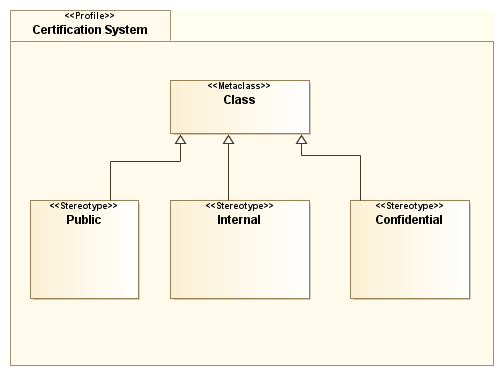
\includegraphics[scale=0.5]{uml/datastereotypes.png}
    \caption{UML wird mit einem Profil um drei Stereotypen erweitert}
\end{figure}

Nach der Erstellung der Stereotypen werden die Daten mit den Vertrautheitskategorien versehen. Sollte es nicht eindeutig sein, welche Klasse in welche Kategorie fällt, müssen die Daten aufgespalten werden und mit einer Assoziation modelliert werden.

\begin{figure}[!htbp]
    \centering
    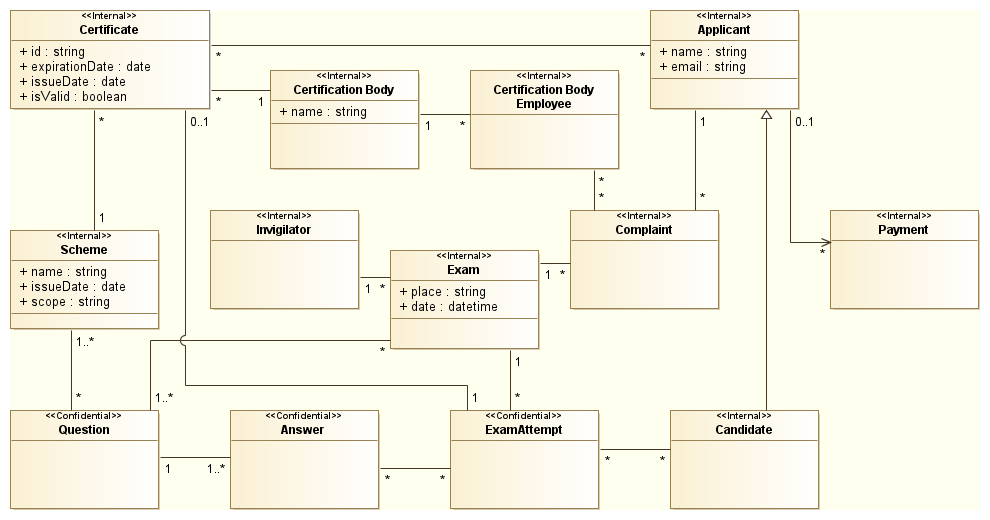
\includegraphics[scale=0.5]{uml/classstereotyped.png}
    \caption{Das Klassendiagramm wird mit Stereotypen der Vertraulichkeit erweitert}
\end{figure}

TODO: datenverlust + angriffsszenarien?

\section{Ermittlung der Akteure und Partnersysteme}
Auf Basis des Usecase Diagrammes können die Akteure und deren Partnersysteme mit Hilfe eines Kontext Diagrammes visualisiert werden

\begin{figure}[!htbp]
    \centering
    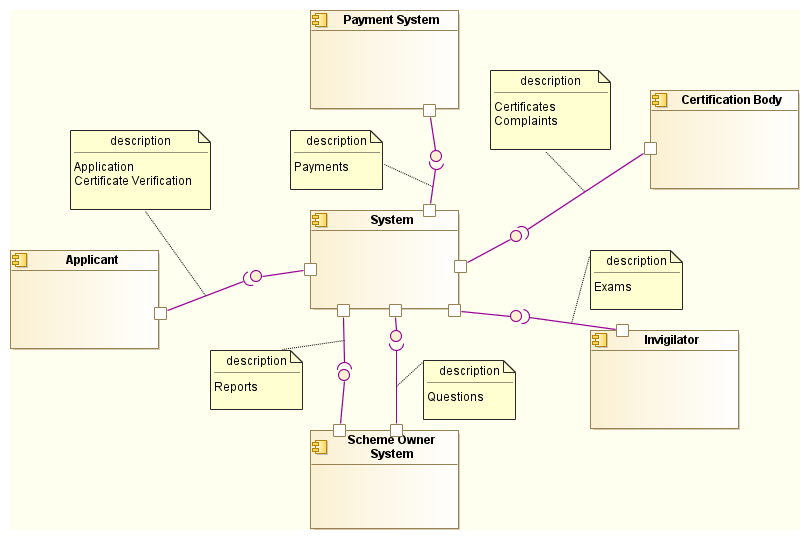
\includegraphics[scale=0.5]{uml/context.png}
    \caption{Das Kontext Diagramm zeigt das System, die Akteure und die Nachbarsysteme}
\end{figure}
\chapter{Erstellung der Architektur}
Aufbauend auf den im Anforderungsprozess ermittelten Attribute, kann nun mit der Architekturplanung begonnen werden. Bereits an dieser Stelle können aufgrund der ermittelten Parameter und Erfahrungswerte eine grundsätzliche Überprüfung der Machbarkeit des Projektes durchgeführt werden. Auch eine Überprüfung, ob der beschriebene Prozess der Architekturplanung für das Projekt eignet kann durchgeführt werden: Der Prozess beschäftigt sich hauptsächlich mit der Aufspaltung und Trennung der Daten und AkteurInnen in mehrere Systeme. Durch außergewöhnlich strenge Laufzeitanforderungen oder entsprechende Rahmenbedinungen kann diese Aufspaltung jedoch zu einer Architektur führen, welche die ursprünglich ermittelten Anforderungen nicht mehr, oder nur schlecht erfüllt.

Die erwähnten Architektursichten werden, soweit möglich, durch UML Diagramme realisert:

\begin{itemize}
  \item Logical View: Klassendiagramm
  \item Process View: Komponentendiagramm, diverse Werte in der Usecasebeschreibung sowie Aktivitäts- und Interface-Klassendiagramm
  \item Development View: Da noch keine Implementation vorhanden ist, können noch keine Bibliotheken und Module beschrieben werden. Hierfür würde sich jedoch das Paketdiagramm anbieten
  \item Physical View: Grobes Komponentendiagramm. Da die Wahl der exakten physischen Komponenten durch die fehlende Implementation nicht früh überprüfbar ist, wurde auf eine Modellierung in der Planungsphase verzichtet
  \item Scenarios: Usecasediagramm
\end{itemize}

\section{Erstellen der minimalen Architektur}
Das Kontextdiagramm, welches im Anforderungsprozess erstellt worden ist, zeigt das System mit allen AkteurInnen und Nachbarsystemen. Aufbauend darauf kann nun die minimale Architektur erstellt werden, welche sich aus dem System und den Nachbarsystemen ableitet.

\begin{figure}[H]
    \centering
    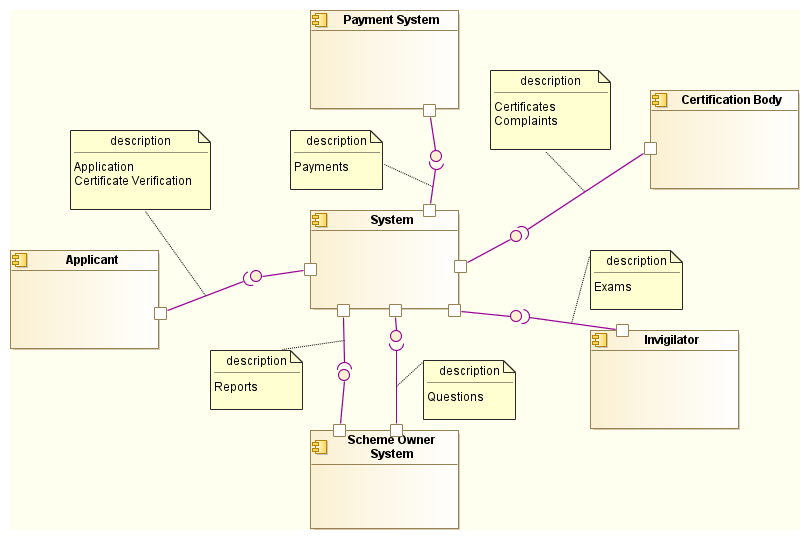
\includegraphics[scale=0.5]{uml/context.png}
    \caption{Das Kontextdiagramm liefert die Ausgangsbasis für die Architektur}
\end{figure}

Zuerst werden alle Datenflussnotizen entfernt. Danach werden alle Komponenten entfernt, welche kein eigenes System darstellen. In diesem Falle werden folgende Komponenten entfernt:

\begin{itemize}
  \item Applicant
  \item Certification Body
  \item Invigilator
\end{itemize}

Dies führt zu folgender Minimalarchitektur:

\begin{figure}[H]
    \centering
    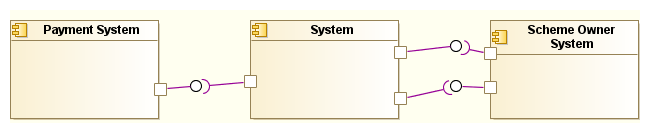
\includegraphics[scale=0.7]{uml/minimalarch.png}
    \caption{Minimale Architektur}
\end{figure}

Für die Nachbarsysteme selbst wird keine Architektur erstellt, jedoch beeinflussen sie die Schnittstellen des Systems und sind deswegen wichtig für den weiteren Prozess. Sie werden in die Architektur einbezogen.

\section{Erstellen der Datenminimalarchitektur}
Auf Basis der im Anforderungsprozess ermittelten Zonen wird das System der vorher erstellte Minimalarchitektur in ebenso viele Teilsysteme unterteilt. Die Aktivitätsdiagramme werden an die neue Architektur angepasst: Für jedes Untersystem wird in den Diagrammen eine eigene Swimlane erstellt. Die involvierten AkteurInnen sind, falls möglich, als eigene Swimlane modelliert, spielen in dieser Phase aber noch keine wichtige Rolle zur Gliederung des Systems.

\begin{figure}[H]
    \centering
    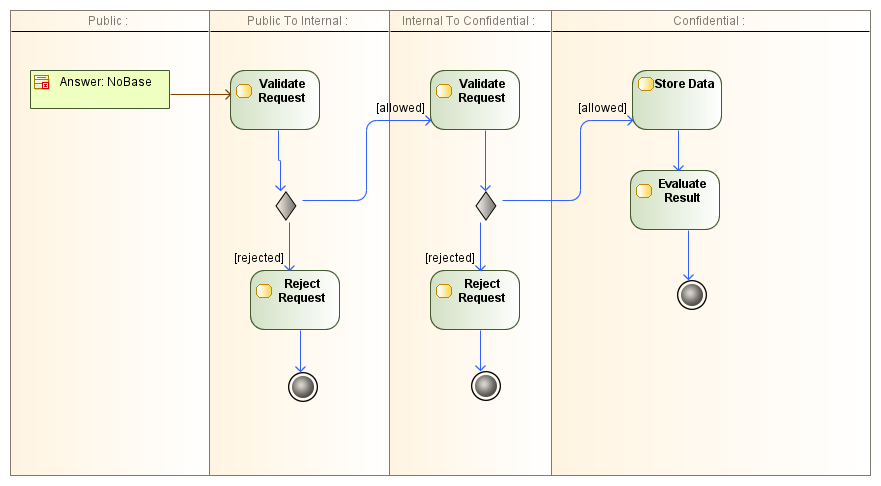
\includegraphics[scale=0.5]{uml/takeexamactivity1.png}
    \caption{Die Antworten werden nach der Prüfung an den Certification Body übermittelt. Der Request wird dann durch zwei Gateways zum finalen System geleitet.}
\end{figure}

Wechselt der Kontrollfluss eine Swimlane eines Systems, heißt dies, dass eine Verbindung zwischen den beiden sonst abgeschotteten Systemen benötigt wird. Dieses Verbindung wird als eigene Komponente modelliert und wird als Gateway bezeichnet. Die Aufgabe dieses Gateways ist es, folgende Attribute der Anfrage zu überprüfen und die Anfrage gegebenenfalls zu verwerfen oder weiterzuleiten:

\begin{itemize}
  \item Von welchem System kommt die Anfrage?
  \item Welches System ist das Ziel der Anfrage?
  \item Welche Schnittstelle dieses Systems ist das Ziel der Anfrage?
  \item Gibt es eine Regel die diese Anfrage explizit erlaubt?
\end{itemize}

Der Gateway fungiert damit als eine Art Application Firewall.

Der Gateway ist jedoch nicht der einzige Punkt an welchem der Zugriff auf Schnittstellen autorisiert wird. Er ist viel mehr ein zusätzlicher Layer, der den Zugriff auf die Schnittstellen absichert. Überwindet ein/eine AngreiferIn durch einen Fehler im Gateway diese Kontrolle, hat er/sie zwar Zugriff zum Internal System, kann aber trotzdem nocht nicht auf die Daten zugreifen, da diese eine zusätzliche Authentifizierung benötigen. \cite{sec}[S. 350]

Die anfangs beschriebenen Nachbarsysteme werden nach ihren Anforderungen, welche aus den Aktivitätsdiagrammen ablesbar sind, an das System in ihrer Zone angeschlossen. Ist das Ausgangssystem ein System, welches nicht vom/von der AuftraggeberIn kontrolliert wird, und greift das Ausgangssystem von einer Zone mit einer niedrigeren Vertrautheitsebene auf ein Zielsystem mit einer höheren Vertrautheitsebene zu, muss dies jedoch über ein zusätzliches System erfolgen. Dies ermöglicht es, den Gateway komplett von unkontrollierten Systemen abzukapseln und dessen Angriffsfläche zu verringern. Dies ist besonders wichtig, weil der Gateway bei Angriffen einen Single Point of Failure darstellt.

Das Beispielprojekt bezieht Zahlungsdaten direkt von einem Payment System und die Prüfungsfragen werden direkt an das Scheme Owner System gesandt. Beides Ausgangssysteme dieser Anfragen stammen aus einem System mit einer höheren Vertrautheitsebene als dem Zielsystem und benötigen deswegen kein eigenes Zwischensystem, sprich können direkt über den Gateway zum Ziel geführt werden. Dem entgegen gesetzt ist die Übermittlung der Prüfungsfragen des Scheme Owner Systems: Das Ausgangssystem greift hier von einem nicht kontrollierten System und einer niedrigeren Vertrautheitsebene auf eine Zielsystem in einer höheren Vertrautheitsebene zu, was eine zusätzliche Komponente nötig macht.

\begin{figure}[H]
    \centering
    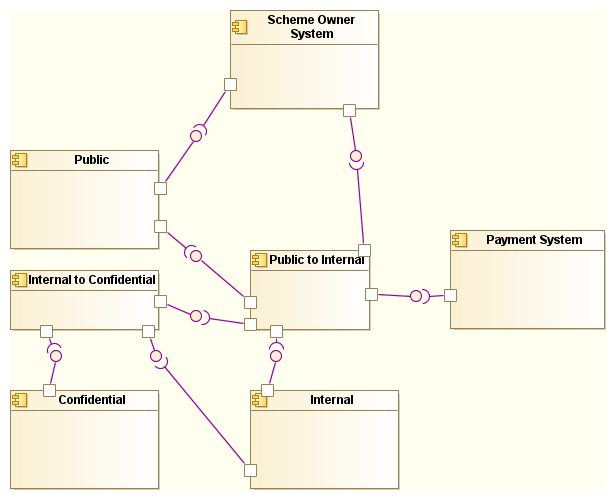
\includegraphics[scale=0.7]{uml/dataarch.png}
    \caption{Aufteilung der Komponenten in Datenbereiche}
\end{figure}

Eine weitere wichtige Regel ist, dass keine Gateways unterschiedlicher Vertrautheitsebenen übersprungen werden dürfen. Zeigt ein Aktivitätsdiagramm zB. einen Zugriff von Ebene 1 auf Ebene 3 muss dieser Zugriff sowohl durch den Gateway der Ebene 2, als auch durch den Gateway der Ebene 3 geleitet werden. Dies verhindert, dass besonders schützenswerte Systeme direkt an Systeme mit einer weitaus niedrigeren Vertrautheitsebene angeschlossen werden und so dessen Gateway zum Single Point of Failure wird. Dies gilt in beide Richtungen.

Da bei der Erstellung des Systems nun alle Schnittstellen und Systeme bekannt sind, können diese Regeln fest im Gateway verankert werden. Weil diese Gateways unabhängig voneinander agieren, können sie durch das Hinzufügen eines Load Balancers beliebig vervielfacht werden, was sowohl die Ausfallsicherheit als auch die Skalierbarkeit erhöht. Das ist wichtig, weil sie als einzige Verbindung zwischen den Systemen zu einer Art Flaschenhals werden.

\section{Einbinden der AkteurInnen}
Nachdem die Datenminimalarchitektur steht, können nun die AkteurInnen des Systems in die Aufgliederung des Systems mit einbezogen werden. Hierfür müssen nun die Objektflüsse und die AkteurInnen des Systems für jeden Usecase betrachtet werden, welche aus den vorher bereits erstellten Aktivitäts- und Kontextdiagramm ersichtlich sind.

Zuerst wird das erste Untersystem, in diesem Falle das Public System, betrachtet. Alle Objektflüsse durch das System und die AkteurInnen, welche mit ihren Swimlanes angrenzen, sind in die Aktivitäten des Systems involviert. Jede Involvierung eines/einer Akteurs/Akteurin in ein System erfordert einen Zugang zu diesem System.

Jeder dieser AkteurInnen muss mit den minimal möglichen Rechten für dieses System ausgestattet werden, um seine Aufgaben zu erfüllen. Dies vermeidet nicht nur Fehler sondern reduziert auch den Schaden, welcher ein potentieller Angriff dieses Akteurs/dieser Akteurin anrichten kann \cite[1. A]{leastpriv}.

Da ein System komplex ist \cite[S. 7]{softarch}, und diese Sicherheitsattribute nach Änderungen am System immer wieder überprüft werden müssen, stellt jeder zusätzliche Zugriff eines/einer Akteurs/Akteurin nicht nur ein Sicherheitsrisiko dar, sondern erhöht auch den Test- und damit den Wartungsaufwand. Idealerweise wird daher jedem/jeder AkteurIn ein eigenes, für sich abgekapseltes System zur Verfügung gestellt, was jedoch meist aufgrund Kosten der zusätzlichen Systeme keine Option dar stellt.

Um zu ermitteln, welche Systeme eine eigene Komponente benötigen, wird nun entweder anhand einer Tabelle oder zusammen mit dem/der KundIn pro Usecase und deren Komponenten ermittelt, ob der Schaden eines unerlaubten Zugriffs der Daten den eines Systems überschreitet. Die Schadens- und Systemkosten müssen zuerst von dem/der KundIn und dem/der ArchitektIn geschätzt werden.

Im Falle des Beispielprojektes wurde auf Basis des folgenden stark vereinfachten Aktivitätsdiagramms in Abbildung \ref{fig:actorarch} ermittelt, dass die möglichen Schadenskosten im Falle, dass der/die AnwärterIn (Applicant) Zugriff auf die Prüfungsantworten (Answer) bekommt, die eines eigenen Systems überschreiten. Das gleiche Problem trifft auch auf den Scheme Owner zu: die Schadenskosten im Falle einer Manipulation oder eines lesenden Zugriffes des/der AnwärterIn (Applicant) auf die Fragen überschreitet auch hier die Kosten eines eigenen Systems. Deswegen werden zwei zusätzliche Systeme erstellt und aus dem Public System ausgegliedert.

Für den Fall, dass bei der Aufspaltung zu viele Systeme entstanden sind, werden nun in einem weiteren Schritt diverse Kombinationen von Teilsystemen betrachtet und versucht zusammen zu legen, solange deren Schadenskosten nicht die Systemkosten überschreiten. Gibt es mehrere mögliche Kombinationen, entscheidet das in den Anforderungen aufgenommene Related Usecases Feld und danach die Überschneidung der Datentypen über die genaue Aufteilung. Ändert sich ein Usecase, so sind meist auch andere Usecases von dieser Änderung betroffen. Je weniger Komponenten nach einer Änderung betrachtet werden müssen, desto niedriger sind die Wartungskosten.

Beim Beispielprojekt zeigt sich, dass es keine erlaubte Kombination gibt, da die Schadenskosten jeweils weit über den Kosten eines eigenen Systemes liegen. Es bleibt somit bei den ermittelten zwei Zusatzsystemen.

\begin{figure}[H]
    \centering
    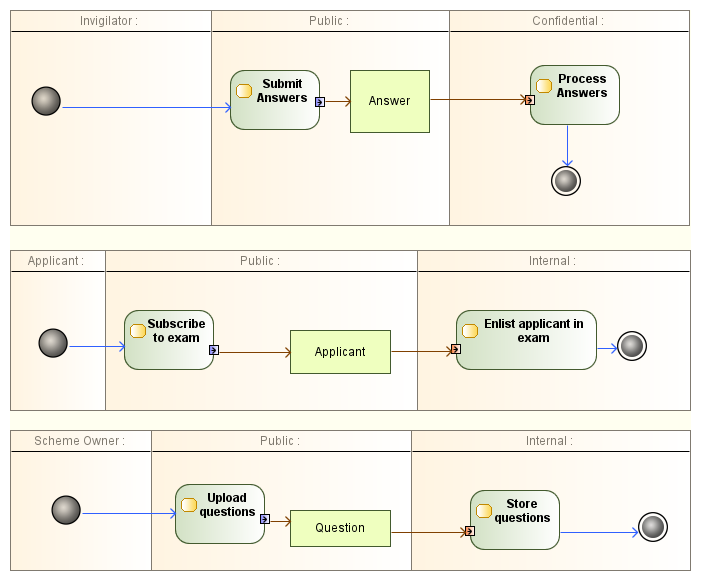
\includegraphics[scale=0.6]{uml/actorarch.png}
    \caption{Vereinfachte Gegenüberstellung von Aktivitätsdiagramme für das Public System}
    \label{fig:actorarch}
\end{figure}

Diese Analyse wird für alle verbleibenden Systeme durchgeführt, bis alle Systeme aufgespalten sind.

Im Falle des Beispielprojektes führt dies schlussendlich zu folgender Systemaufspaltung:

\begin{figure}[H]
    \centering
    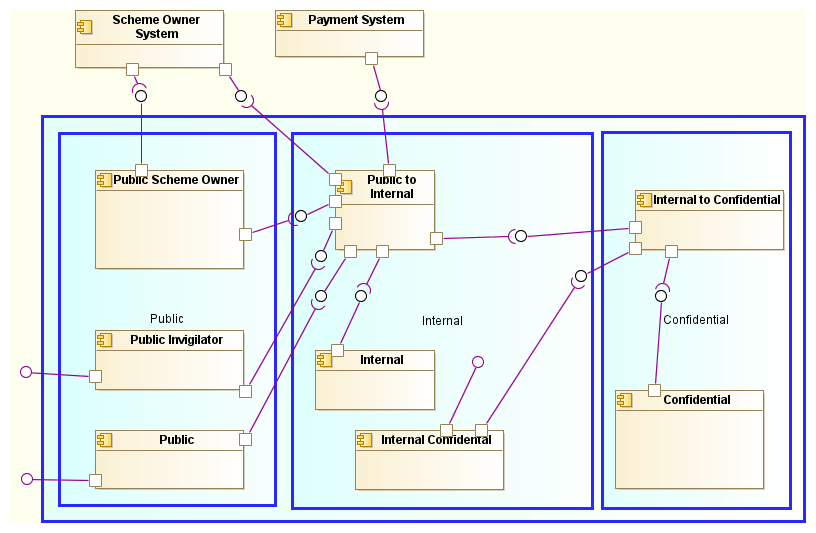
\includegraphics[scale=0.6]{uml/vision4.png}
    \caption{Architektur nach der Aufspaltung }
\end{figure}

\section{Analyse der nicht funktionalen Attribute}
Ist die erste Version der Architektur erstellt, kann nun mit der grundsätzlichen Überprüfung der im Anforderungsprozess ermittelten Parameter begonnen werden, welche bereits wichtige Informationen und Rückschlüsse auf den jetzigen Status der Architektur geben. Basierend auf den Usecases, den ermittelten Komponenten der Architektur und den Aktivitätsdiagrammen wird eine Tabelle erstellt, welche Auskünft darüber gibt, welche Komponenten für jeden Usecase benötigt werden. Diese Tabelle dient als Basis für weitere Analysen.

Um herauszufinden, welche Komponenten für einen Usecase benötigt werden, können die Swimlanes der Aktivitätsdiagramme herangezogen werden. Da für AkteurInnen keine Komponente gelistet werden, werden deren Swimlanes ignoriert. Ein Beispiel hierfür ist das Aktivitätsdiagramm des Handle Complaint Usecases in Abbildung \ref{fig:handlecomplaintreview}.

\begin{figure}[H]
    \centering
    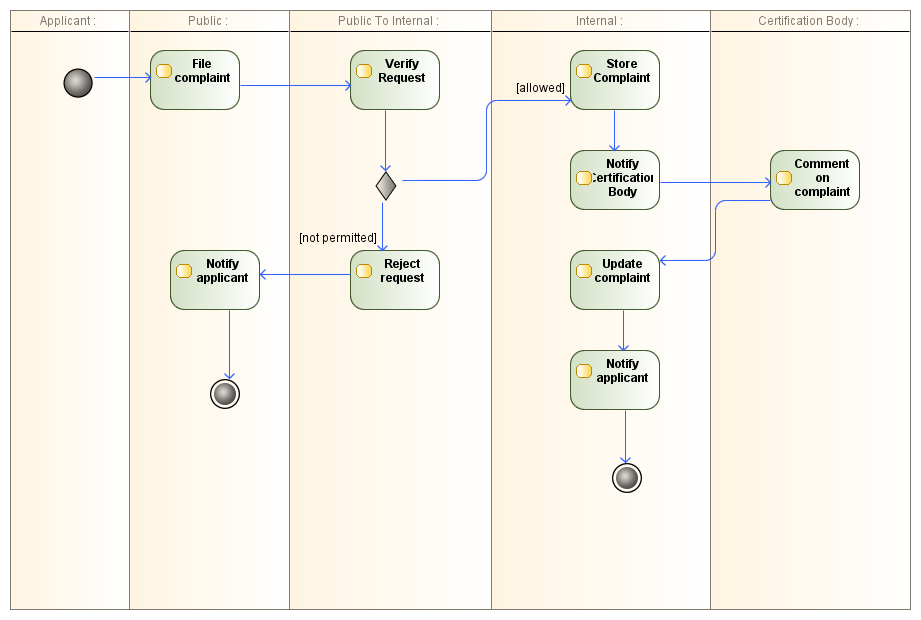
\includegraphics[scale=0.5]{uml/handlecomplaintsactivityreview.png}
    \caption{Vereinfachtes Aktivitätsdiagramm des Handle Complaints Usecases mit der id complaints}
    \label{fig:handlecomplaintreview}
\end{figure}

Werden die beiden AkteurInnen entfernt, bleiben für diesen Usecase folgende Komponenten übrig:

\begin{itemize}
  \item Public
  \item Public To Internal
  \item Internal
\end{itemize}

Diese werden nun in eine Tabelle überführt, wobei für jede verwendete Komponente eines Usecases mit einem x markiert wird:

\hfill \break

\begin{tabular}{ | r | c | }
    \hline
    Komponenten & complaints \\
    \hline
    Public & x \\
    \hline
    Public Invigilator & \\
    \hline
    Public Scheme Owner & \\
    \hline
    Public To Internal & x \\
    \hline
    Internal & x \\
    \hline
    Internal Confidential & \\
    \hline
    Internal To Confidential & \\
    \hline
    Confidential & \\
    \hline
    Scheme Owner System & \\
    \hline
    Payment System & \\
    \hline
\end{tabular}

\hfill \break

Dies wird für alle Usecases durchgeführt und führt im Falle des Beispielprojektes zu folgender Matrix:

\begin{figure}[H]
    \centering
    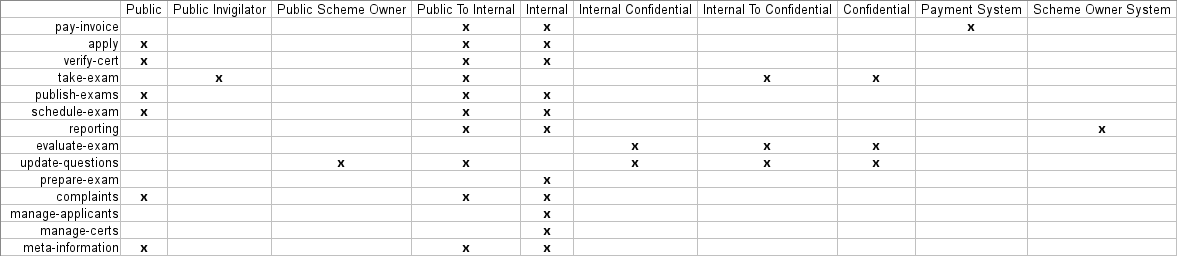
\includegraphics[scale=0.4]{img/matrix.png}
    \caption{Matrix der Komponenten und Usecases des Beispielprojektes}
    \label{fig:matrix}
\end{figure}




\subsection{Reliability}
Anhand der in ermittelten Usecase und Komponenten Matrix kann nun sowohl eine Überprüfung der der Ausfallskosten als auch eine Single Point of Failure Analyse durchgeführt werden.

\subsubsection{Single Point of Failure Analyse}

Ein Single Point of Failure beschreibt eine Komponente, die so kritisch für das System ist, dass ihr Ausfall den kompletten Ausfall des Systems nach sich zieht \cite[S. 3]{single}. Ein Single Point of Failure der Architektur kann daran erkannt werden, dass eine Komponente in allen Usecases vorkommt. Im Bezug auf die soeben ermittelte Matrix wird dies durch eine durchgehende Reihe von mit x markierten Zellen in der Komponentenspalte ersichtlich.

Enthält eine Architektur einen Single Point of Failure, muss diese Komponente entweder redundant ausgelegt sein, oder es muss eine Aufspaltung anhand einer Fehlerkostenanalyse durchgeführt werden.

Im Falle der Matrix in Abbildung \ref{fig:matrix} ist keine durchgehende Reihe an markierten Zellen erkennbar und somit existiert kein Single of Failure. Es lässt sich einzig und allein ablesen, dass die Public To Internal und Internal Komponente eine Abweichung vom Single Point of Failure um vier respektive drei besitzen. Dies lässt erahnen, dass bei der Implementation und Wartung dieser Systeme besondere Sorgfalt von Nöten ist.

\subsubsection{Ausfallkosten Analyse}
Zusätzlich zu einer Single Point of Failure Analyse gibt eine Ausfallkosten Analyse auf Basis des in den Anforderungen ermittelten Monatsumsatzes Auskunft darüber, welche Komponenten jeweils wieviel Umsatz generieren. Für diese Überlegung können auch die Wachstumsszenarien einbezogen werden, falls sich der Umsatz durch eine Steigerung der BenutzerInnen steigert oder senkt.

Das Ergebnis dieser Analyse ist die notwendige Redundanz der einzelnen Komponenten, welche bei der Implementation des Systems erreicht werden muss.

Die nachfolgenden Berechnungen verteilen den Schaden aus Gründen der Einfachheit gleichmäßig auf alle Zeiteinheiten. Es kann sein, dass eine Organisation so strukturiert ist, dass ein eintägiger Ausfall keine Umsatzeinbußen nach sich zieht. In diesem Falle ist die Beispielrechung ungenau. Um diese Möglichkeit einzubeziehen, müssen detailiertere Umsatzkosten im Anforderungsprozess ermittelt werden was jedoch aus Gründen des Umfangs und der Einfachheit vermieden wird. Das Beispiel soll lediglich als ein anschauliches Beispiel zur Ermitllung des Umsatzrückganges dienen.

Um den monatlichen Umsatz der Komponenten zu ermitteln, wird das x in den markierten Feldern mit dem Monatsumsatz des Usecases ersetzt. Leere Felder werden mit 0 aufgefüllt. Schlussendlich werden alle Werte einer Komponente addiert, um den Gesamtumsatz zu ermitteln.

Als Beispiel dient hier die Internal Komponente (Die Werte sind beispielhaft gewählt):

\hfill \break

\begin{tabular}{ | r | c | }
    \hline
    Usecases & Internal \\
    \hline
    pay-invoice & 3000 \euro \\
    \hline
    apply & 1500 \euro \\
    \hline
    verify-cert & 1500 \euro \\
    \hline
    take-exam & 0 \euro \\
    \hline
    publish-exams & 1500 \euro \\
    \hline
    schedule-exam & 1500 \euro \\
    \hline
    reporting & 1500 \euro \\
    \hline
    evaluate-exam & 0 \euro \\
    \hline
    update-questions & 0 \euro \\
    \hline
    prepare-exam & 80000 \euro \\
    \hline
    complaints & 1500 \euro \\
    \hline
    manage-applicants & 1500 \euro \\
    \hline
    manage-certs & 1500 \euro \\
    \hline
    meta-information & 1500 \euro \\
    \hline
    Total Sum & 96500 \euro \\
    \hline
\end{tabular}

\hfill \break

Fällt diese Komponente für einen kompletten Monat aus, verursacht sie einen Umsatzrückgang von 95500 \euro. Wenn eine Komponente eine Ausfallwahrscheinlichkeit von 99\% besitzt, dann belaufen sich die durchschnittlichen Ausfallkosten auf 965 \euro. Wird aus Redundanzgründen eine weitere Komponente hinzugefügt und damit die Ausfallwahrscheinlichkeit auf zB. 99.9\% gesteigert, belaufen sich die Schadenskosten nur noch auf 96.5 \euro. Kostet diese zusätzliche Komponente weniger als die Differenz der Kosten, sprich weniger als 868.5 \euro, rentiert sich die Anschaffung einer zweiten Komponente.

\subsection{Usability}
Da die Artefakte des Planungsprozesses keine Oberflächen beschreiben ist eine Auswertung der des nicht funktionalen Parameters Usability nicht möglich. Außerdem ist sie nicht im Fokus der Architekturerstellung und die Überprüfung der Usability kann somit übersprungen werden.

\subsection{Efficiency}
Es ist schwierig, die Effizienz und Performance der Architektur in diesem Stadium zu messen, da noch keine Implementation vorhanden ist und somit weder die Performance noch der Speicherverbrauch des Systems getestet werden können. In diesem Stadium lassen sich lediglich Werte schätzen. Eine Möglichkeit um zB. die Antwortzeiten zu schätzen, ist es, die Anzahl der Swimlanewechsel eines Usecases zu addieren und das Ergebnis mit einer konstanten Zeit, welche auf Erfahrungswerten basiert, zu multiplizieren. Dieser Wert kann dann mit den im Anforderungsprozess ermittelten Antwortzeiten verglichen werden, um zu überprüfen, ob das System diese Anforderungen erfüllt.

Ausgegangen wird hier von den bestehenden Aktivitätsdiagrammen. Je nachdem, für welchen Abschnitt die in den Anforderungen ermittelten Werte gelten, kann nicht der komplette Ablauf des Aktivitätsdiagrammes für die Berechnung der Zeit verwendet werden.

Überschreitet der berechnete Wert den in den Anforderungen ermittelten Wert, muss dessen Kategorie hinzugezogen werden. Ist der Wert nur eine Empfehlung, so wird der Usecase in der Implementationsphase mit einem besonderen Augenmerk auf Geschwindigkeit umgesetzt. Ist der Wert jedoch verbindlich, so muss mit dem/der KundIn Rücksprache gehalten werden \cite[S. 70]{effektiv}: Entweder ist die Anforderung unter diesen Parametern nicht umsetzbar, oder es muss ein Kompromiss zu lasten von anderen Anforderungen eingegangen werden.

Ein Beispiel für die Berechnung der Antwortzeiten wird aus dem Aktivitätsdiagramm des Beispielprojektes für die Anmeldung eines Kandidaten erläutert (Abbildung \ref{fig:applycomplicated}):

\begin{figure}[H]
    \centering
    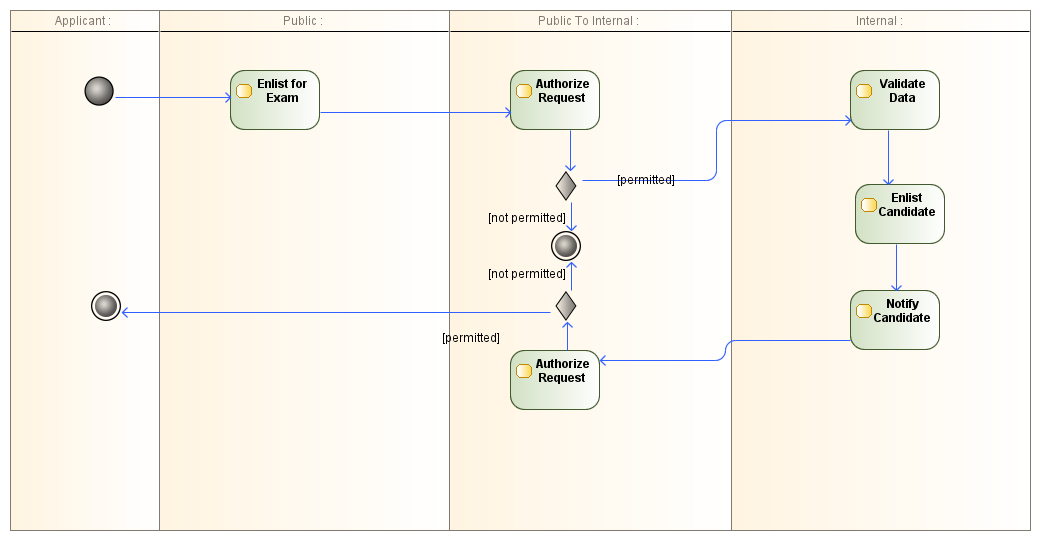
\includegraphics[scale=0.4]{uml/applycomplicated.png}
    \caption{Der Kandidat meldet sich für eine Prüfung an}
    \label{fig:applycomplicated}
\end{figure}

Hier werden, ausgegangen vom Startpunkt sechs Swimlanewechsel gezählt. Diese werden nun mit der Konstante 100 Milisekunden multipliziert, was eine geschätzte Durchlaufzeit von 600 Milisekunden ergibt. Dies liegt unter den erforderlichen 1000 Milisekunden der aufgenommenen nicht funktionalen Anforderung der Antwortzeit.

\subsection{Maintainability}
Maintainability dreht sich um Wart- und Änderbarkeit eines Projektes. Die Änderbarkeit der Architektur hängt wesentlich von der Kopplung und Kohäsion der Komponenten ab. Die Wartbarkeit kann unter anderem an den Wartungskosten abgelesen werden.

\subsubsection{Kopplung und Kohäsion}
Die Änder- und Wartbarkeit ist wesentlich von den Beziehungen der Komponenten und Usecases abhängig. Wird eine Komponenten geändert, so müssen zusätzlich zu dieser Änderung auch eine erneute Validierung der bereits bestehenden Funktionen durchgeführt werden, um Fehler, welche aus den Änderungen entstanden sind, zu finden. Dieses Problem wird mit dem Begriff Ripple Effect beschrieben. \cite[S. 3]{ripple}

Wird ein Usecase geändert, so müssen eine oder mehrere Komponenten des Usecases angepasst werden. Wird eine Komponenten geändert, so kann dies auch andere Usecases beeinflussen, welche die gleiche Komponente verwenden. Wie sehr eine Komponente andere Usecases beeinflusst, kann aus den Komponenten Spalten der Matrix abgelesen werden, in dem die Anzahl der mit x markierten Spalten durch die Anzahl der Gesamtusecases dividiert wird. Der daraus resultierende Wert liegt in den Grenzen von 0 (bester Wert) und 1 (schlechtester Wert) und gibt die Kopplung der Komponente an. \cite[S. 164]{effektiv}

Die Kohäsion beschreibt die inhaltliche Zusammengehörigkeit der Komponenten \cite[S. 164]{effektiv}. Sie kann aus den der Usecase-, Aktivitäts und Klassendiagrammen ermittelt werden. Das Klassendiagramm beschreibt die Zusammengehörigkeit der Daten, das Aktivitätsdiagramm eines Usecases und dessen Objektflüsse die gemeinsam verwendeten Daten. Die Usecases können nun anhand der verwendeten Daten in mehrere unabhängige Gruppen unterteilt werden, die orthogonal zueinander sind. Je mehr unabhängige Gruppen auf eine Komponente zugreifen, desto schlechter ist deren Kohäsion.

Zusätzlich können nun die in den Anforderungen ermittelten Änderungsszenarien mit einbezogen werden. Hat eine Komponente einen hohen Kopplungswert und/oder eine niedrigen Kohäsion, und ist sie Teil eines Usecases, welcher viele Änderungsszenarien beinhaltet, kann dies als Grund zu einer weiteren Aufspaltung der Komponente genommen werden. Gateways sind von Aufspaltungen ausgenommen, da sie als Firewall agieren und so simpel wie möglich konfiguriert werden müssen, um Konfigurationsfehler zu vermeiden.

Wird eine Aufspaltung durchgeführt, so werden sie anhand der in Kohäsionsanalyse ermittelten Gruppen aufgeteilt. Die Priorität der Gruppen wiederum ergibt sich aus den ermittelten Änderungsszenarien, danach werden die in der Ausfallskostenanalyse ermittelten Kosten einer Komponente herangezogen. Diese Ordnung ergibt sich aus der Erkenntnis, dass die Wartung der Software oft mehr als 50\% der Gesamtsystemkosten des Systems ausmacht \cite[S. 71-84]{maincost}.

Die Änderungsszenarien und die Kopplungswerte stellen schlecht bewertbare Werte dar. Zudem kann eine feste Aufteilung anhand der unabhängigen Gruppen der Kohäsion zu einem System führen, in welchem jeder kleine und unabhängige Usecase ein eigenes System bekommt, was wiederum zu einer zu starken Fragmentierung führen kann. Deshalb kann hier keine starre Regel festgelegt werden, wann ein System aufgespalten werden muss und wann nicht. Diese Entscheidung muss vom/von dem/der ArchitektIn selbst getroffen werden.

Wird das Beispielprojekt auf Kohäsion und Kopplung analysiert, fallen vor allem die Internal und Public To Internal Komponente auf, da sie in mehr als der Hälfte aller Usecases eingesetzt werden (Kopplungswert größer als 0.5). Weil die Public To Internal Komponente ein Gateway ist, kann sie ignoriert werden. Damit verbleibt die Internal Komponente. Wird die Kohäsion der Internal Komponente betrachtet, sticht hervor, dass in dieser Komponente mehrere komplett unabhängige Daten verwendet werden: Zahlungen, Zertifikate, Anmeldungen und Beschwerden sind jeweils eigene, logische Gruppen.

Aufgrund der Größe des Systems und der wenigen Änderungsszenarien wurde gegen eine weitere Aufspaltung entschieden, jedoch wurde fest gestellt, dass die Internal Komponente bei der Erstellung der Testfälle eine höhere Testabdeckungen benötigt.

\subsubsection{Wartungskosten}
Die Wartungskosten ergeben sich sowohl aus dem Personal, welches für die Wartung der Komponenten angestellt werden muss, als auch aus den Strom- und Reparaturkosten der eingesetzten Systeme. Weil die genauen Komponenten noch nicht implementiert wurden, kann an diesem Moment nur eine Schätzung der Kosten durchgeführt werden.

Eine einfache Möglichkeit zur Schätzung der Kosten kann durch die Wahl einer Konstanten pro System durchgeführt werden. Im Falle des Beispielprojektes wird pro System mit folgenden monatlichen Kosten gerechnet:

\begin{itemize}
  \item Stromkosten: 10 \euro
  \item Reparaturkosten: 20 \euro
  \item Personalkosten: 100 \euro
\end{itemize}

Die aufsummierten Kosten ergeben Wartungskosten von 130 \euro \ pro Monat. Wird dies mit der Anzahl der Systeme multiplizert ergibt sich ein Gesamtwartungskostenaufwand von 8 * 130 \euro, sprich 1040 \euro \ pro Monat.

\subsection{Portability}
Die Portabilität der Platform kann im Moment noch nicht überprüft werden, da noch keine Festlegung des Projektes auf eine Plattform und/oder Technologie existiert. Dies kann erst zu Beginn der Implementationsphase entschieden werden und wird unter anderem von den in der Anforderungsphase ermittelten Rahmenbedingungen beeinflusst.


\section{Modellierung der Komponentenschnittstellen}
Sind alle Analysen der Architektur abgeschlossen, kann nun anhand der Usecase-, Klassen und Aktivitätsdiagramme damit begonnen werden, die Schnittstellen der Komponenten zu definieren. Die Schnittstellen werden als Interfaces in einem Klassendiagramm modelliert und schlussendlich in das Komponentendiagramm integriert.

Um die unterschiedlichen erlaubten Zugriffe zu modellieren, kann Vererbung genutzt werden: gemeinsame Schnittstellen werden in eine Basisklasse ausgelagert. Obwohl der Gateway bereits einen Großteil der Zugriffe regelt, sind wie in Kapitel 7.2 beschrieben zusätzliche Überprüfungen der Zugriffe von Nöten. Eine Visualisierung dieser verschiedenen Zugriffsrechte ist somit von Vorteil.

Ein Beispiel dafür ist die Beschwerdenschnittstelle des Beispielprojektes, welches sowohl eine Interne als auch eine Public Schnittstelle anbietet. Beide Schnittstellen haben gemeinsame Operationen, welche mit Vererbung modelliert wurden.

\begin{figure}[H]
    \centering
    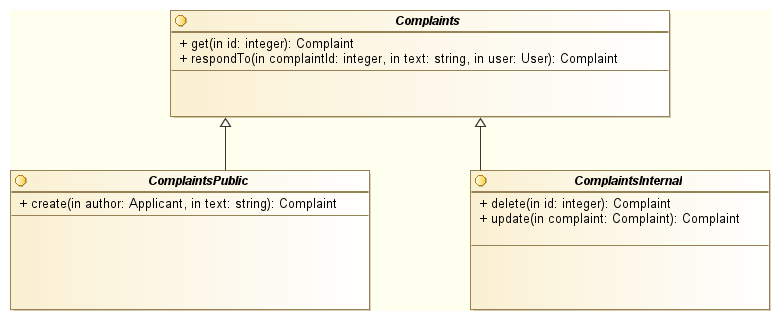
\includegraphics[scale=0.6]{uml/complaintsinterface.png}
    \caption{Erstellen der Verschiedenen Complaints Interfaces}
\end{figure}

Die verschiedenen Schnittstellen können nun in das Architekturkomponentendiagramm integriert werden. Dies wird für alle Komponenten durchgeführt und schließt die Architekturplanungsphase ab.

Nun kann mit der Implementierungsphase begonnen werden, welche sicht nicht nur mit der Technologie, sondern auch der Programmstruktur beschäftigt. Die Implementierungsphase aus Gründen des Umfangs nicht mehr Teil dieses Prozesses.

\begin{figure}[H]
    \centering
    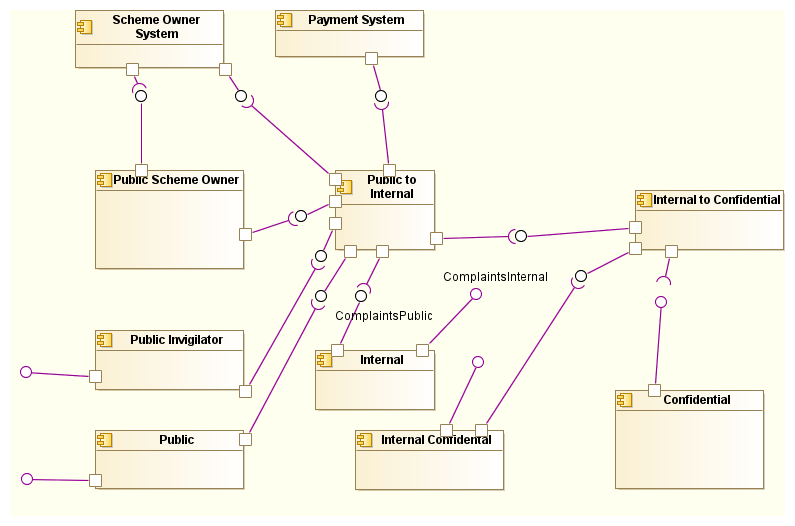
\includegraphics[scale=0.6]{uml/v5.png}
    \caption{Verlinken der Complaints Schnittstelle}
\end{figure}

\section{Changemanagement}
Je nachdem ob noch möglich/gewünscht aufzeigen wie würde ein Change request ausschauen, z.B. was wäre nötig um einen zusätlichen Typ User des Systems einzubinden


\chapter{Zusammenfassung}

\section{Warum ist der Prozess gut}
\subsection{10er Regel der Fehlerkosten}
\subsection{Minimiert Angriffsfläche für wichtige Infrastruktur}
\subsection{Fokus Datensicherheit}
\subsection{Lässt Entscheidungen aufschieben}
\subsection{Kochrezept lässt sich ableiten}
\subsection{Wichtige Anforderungsparameter schon früh einbezogen}
\subsection{Visuelle Repräsentationen mit denen schnell bewertet werden kann}

\section{Limitierungen}
\subsection{Benötigt noch mehr Input von anderen Projekten}
da beispielprojekt wegen den anforderungen starken wert auf datensicherheit legt und deswegen architektur prozess beinflusst hat

\subsection{Nicht alle nicht funktionalen Anforderungen überprüfbar}
Sprich es ist bis zu einem gewissen Teil möglich
\subsection{Problem wenn sicht Akteure/Daten oft ändern}
\subsection{Zum Teil auch abhängig von Erfahrungswerten}
\subsection{Nur Plangungsphase, ohne Implementierungsphase}
\subsection{Extremarchitekturen}

\section{Erkenntnisse}
\subsection{Ohne messbare Parameter kein Kochrezept möglich}
\subsection{Parameter nicht zu jeder Phase messbar}
\subsection{Priorisierung von nicht funktionalen Parametern schwer möglich}
\subsection{Generische Komponentenarchitektur durch viele und schnell ändernde Kombinationen schwer möglich}
\subsection{Auf Ehrfahrungswerte kann nicht vollkommen verzichtet werden}
\subsection{Funktionale Anforderungen beeinflussen Archtitektur mehr als gedacht}
Prozess erstellt die frühe Architektur hauptsächlich durch einbeziehen funktionaler parameter, nicht funktionale parameter wegen fehlender implementation schwer messbar.

\section{Ausblick}
Prozess in der Planungsphase erprobt. Implementierungsphase auch wichtig, aber nicht beschrieben. Nächste Schritte könnten sein den Prozess mit einer Implementierungsphase zu erweitern. 1 Projekt hat viele Probleme schon aufgezeigt, aber weitere, unterschiedliche Projekte wären gut um den Prozess noch zu verbessern.

\clearpage
\bibliographystyle{gerabbrv}
\bibliography{Literatur}
\clearpage

% Das Abbildungsverzeichnis
\listoffigures
\clearpage

% Das Tabellenverzeichnis
\listoftables
\clearpage

% Das Quellcodeverzeichnis
\listofcode
\clearpage

\phantomsection
\addcontentsline{toc}{chapter}{Abkürzungsverzeichnis}
\chapter*{Abkürzungsverzeichnis}
\begin{acronym}[XXXXX]
    \acro{VPN}[VPN]{Virtual Private Network}
    \acro{CRUD}[CRUD]{Create Read Update Delete}
    \acro{ATAM}[ATAM]{Architecture Trade-off Analysis Method}
    \acro{CBAM}[CBAM]{Cost Benefit Analysis Method}
    \acro{ROI}[ROI]{Return of investment}
    \acro{WWW}[WWW]{world wide web}
\end{acronym}
\clearpage

\phantomsection
\addcontentsline{toc}{chapter}{Anhang}
\chapter*{Anhang}


\end{document}
